
\section{Magnitude relations, MAG} 

The MAG program\index{MAG} calculates simple \index{Magnitude relation}magnitude relations. The program has three functions: (1) Calculate parameters for a magnitude scale (\index{Ml}Ml or \index{Mc}Mc), (2) Calculate relation between two different magnitudes and/or spectral parameters and (3) Calculate a new magnitude as a function of an existing magnitude, a natural step following function (2). All three functions can be done at the same time. Function (3) can also be used for moving a particular magnitude type and/or agency to the first magnitude position in line 1 to be plotted with EPIMAP. \index{Magnitude} 

ALL HEADER LINES ARE SEARCHED FOR MAGNITUDE INFORMATION 

Input: The data input is a CAT-file like one made with SELECT or COLLECT or it can be a compact file if only magnitude comparison is made. Optionally there can be a parameter file, which MUST be, called mag.par and MUST reside in the working directory. An example of the parameter file is found in DAT and also shown below. The parameter file is not needed for all operations, see details below. 

1: Magnitude scales 

Coda magnitude Mc: The coda magnitude scale used is 

\begin{displaymath}
Mc = A * log(coda) + B * dist + C 
\end{displaymath}

where \index{Mc}Mc is the coda magnitude, coda is the \index{Coda length}coda length in secs, dist is the hypocentral distance in km (calculated from epicentral distance and depth in CAT file) and A, B and C are constants to be determined. This is done in two ways 

3d regression 

\begin{displaymath}
m = A * log (coda) + B * dist + C 
\end{displaymath}

2d regression 

\begin{displaymath}
m = A * (log (coda) + dist\_coff * dist) + C 
\end{displaymath}

with B = A * dist\_coff where dist\_coff is given in the parameter file and m is the reference magnitude. SO B AND dist\_coff ARE DIFFERENT. The CAT-file must contain coda readings, epicentral distances and a magnitude in the header line. A linear regression is then made between the known magnitude from a given agency and the observed coda lengths following the relations above. The user has the option to choose the type of magnitude to use in the regression. Usually Ml or Mb are used. All station-event combinations are used to determine simultaneously the 3 constants A, B and 
C. Since the data often is too bad to determine all 3 parameters at the same time, the program will also calculate just A and C using a fixed user supplied value for the distance correction to the coda. 
The constant dist\_coff is given in the mag.par file as the second parameter under MAG\_TYP\_COF (see below). IN ORDER FOR THE CODA SCALE OPTION TO WORK, THE DISTANCE COEFFICIENT MUST BE DIFFERENT FROM ZERO. 

Output: On the screen the constants will be printed out and a file mag\_coda.out will contain pairs of values m and (log(coda) + dist\_coff*dist), which can be used to plot the distance corrected coda relation. If results from the 3D is to be plotted, dist\_coff must be calculated as dist\_coff=B/A, put into mag.par and mag run again. On the other hand, if a best dist\_cof has been found, B is calculated as B=A*dist\_cod 

A typical coda magnitude relation is :

\begin{displaymath}
Mc = 2.0*log(coda) + 0.0035*dist - 0.87 
\end{displaymath}
\citep{lee1972} 

Local magnitude \index{Ml}Ml: \newline
The local magnitude scale is calculated by determining an amplitude attenuation scale using amplitudes and distances in CAT file. The parameters in the Ml magnitude scale are computed for every event individually, parameters are determined as averages of all events. 

For each event (only type L and R are used) a,b,c are calculated if at least 3 stations are available 
using least squares regression as follows: 

\begin{displaymath}
log(amp) = a * log(dist) + b * dist + c \index{Amplitude attenuation}\index{Quality factor} 
\end{displaymath}

The relation above can be derived from the standard geometrical spreading and attenuation relations: 

\begin{displaymath}
amp = (dist ** a) * exp(pi * f * dist/(v*q )) 
\end{displaymath}

where $f$ is the frequency, $v$ is the velocity and $q = q0*f**qalpha$. The relation can be rewritten 

\begin{displaymath}
log(amp) = a * log(dist) + (pi * f * dist) /(v * q0*f**qalpha * 2.3) 
\end{displaymath}

Since $qalpha$ often is close to $1.0$, the relation can be simplified to the frequency independent relation:

\begin{displaymath}
log(amp) = a * log(dist) + (pi * dist) /(v * q0 * 2.3) 
\end{displaymath}

If body wave spreading is assumed $(a=1)$, $q0=100$ and $v=3.5 km/sec$, the relation is 

\begin{displaymath}
log(amp) = 1.0 * log(dist) + 0.004 * dist 
\end{displaymath}

which is comparable to the relation shown below for California. 

Similarly to the coda relation, a 2D relation is also calculated 

\begin{displaymath}
log(amp) - b*dist = a * log(dist) 
\end{displaymath}

where $b=dist\_coff$ is fixed to the value given in the mag.par file (same parameter as used for coda). This gives a more stable solution, however b = dist\_coff must be determined by trial and error or fixed using known values from e.g. q-studies.\index{Geometrical spreading} 

The amplitudes are assumed to be ground displacements (in SEISAN they are \index{Ground displacement}ground displacements highpass filtered at 1.25 Hz to resemble \index{Wood Anderson}Wood Anderson seismograms, see MULPLT). The distance ratio between stations with the maximum distance and minimum distance must be more than 3 for the event to be selected for analysis. It is assumed that a and b will be the same for all events, while c is different (magnitude dependent). At the end, the average constants a and b are calculated of all values a and b which are not deviating too much (a must be in the range 0 to -5, hardwired). Distance attenuation coefficients a and b are supposed to be negative since amplitude decrease with distance. To get the \index{Local magnitude}local magnitude scale 

\begin{displaymath}
Ml = log(amp) - a * log(dist) - b * dist - C 
\end{displaymath}

the constant C must be determined by fixing the magnitude at some 
reference distance like the original Wood Anderson definition with 
$Ml = 3$ at $dist= 100 km$ and $amp=1/2200 mm = 454 nm$ (assuming gain of 
the Wood Anderson seismograph to be 2080, \citep{hutton1987}. 
The determination of a and b does not work well unless the observations 
are very good. The relation for California is \citep{hutton1987}

\begin{displaymath}
Ml = log(amp) + 1.1 *log(dist) + 0.00189 * dist - 2.09 
\end{displaymath}

Output: On the screen the constants will be printed out and a file mag\_amp.out will contain the values of a, b and c. 

2: Magnitude relations and/or spectral parameter relations 

Linear regression (maximum likelihood) can be made between any two magnitudes and/or spectral parameters on any of the header lines of an event in a CAT-file or a compact file. The user is interactively prompted for the magnitude type and/or spectral parameters and agencies to compare. If none is given, no magnitude comparison will be made. If several magnitudes/spectral parameters fit the requirement, the last one is used. If e.g. the first header line has a BER Ml and the last header line also has a BER Ml, the last one will be used.  Maximum likelihood linear fitting is used. It is assumed that both variables have normal and correlated errors. See subroutine maxlik.for in LIB for more info. 

The following parameter can be selected: 

Any magnitude and agency \newline
Seismic moment(log) \newline
Stress drop (log) \newline
Corner frequency (log) \newline
Source radius(log) \newline
Spectral decay \newline
Omega zero level (log) 

If any of the spectral parameters are selected, or  moment magnitude is without agency, there will be an additional question about which station and component. A blank return means the average will be used. With these parameter selections, it is possible to compare spectral parameters from any two channels, compare the average spectral parameter with the parameter from one channel etc. 

Output: A plot will be shown on the screen with the observations and the least squares fit and the values are also printed out on the screen. A file mag\_mag.out contains the pairs of magnitudes used. 

3: \index{Magnitude conversion}Magnitude conversions 

If a relation between two magnitude scales is known, e.g. by using option 2 above, an output file can be made with the \index{Converted magnitude}converted magnitudes. The relation to use is specified in the mag.par file. Several different input magnitude types and agencies can be used and the relation-agency used is given in a priority list in the mag.par file, see example below. It is here shown that if a BER Mc is available, this will be the first choice. If no BER Mc then BER Mb will be the next choice etc. The new magnitude will have type X and \index{Agency}agency NEW. Output: The output file is mag\_new.out and has the same format as the input file. On the header line, the old magnitudes are removed and in the first magnitude position will be the converted magnitude (NEW) while in the second magnitude position, the magnitude selected for \index{Mag\_amp.out}\index{Mag\_coda.out}\index{Mag\_mag.out}\index{Mag\_new.out}\index{Mag\_newa.out}\index{Mag\_spec.out}\index{Spectral parameters}conversion will be given. The third magnitude position is blanked out. The conversion option can also be used to move magnitudes around by using a 1 to 1 relation as shown in mag.par example. 

Summary of output files: 

\begin{tabular}{lp{10cm}}
\texttt{mag\_amp.out} : & Details each event for amplitude regression. \\
\texttt{mag\_coda.out} : & Magnitude vs coda, see text. \\
\texttt{mag\_mag.out} : & Pairs of magnitudes used for regression. \\
\texttt{mag\_new.out} : & Events with converted magnitudes only. \\
\texttt{mag\_newa.out} : & All events, both converted and non converted (due to no correct input     magnitude available). \\
\texttt{mag\_spec.out} : & Summary of normal header line, all associated magnitudes    and spectral parameters. \\
\texttt{mag\_ml\_inv.out} : & From Ml inversion \\
\end{tabular}

In DAT there is an example \texttt{mag.par} file. 

\begin{figure}
\htmlimage{scale=2.0}
\centerline{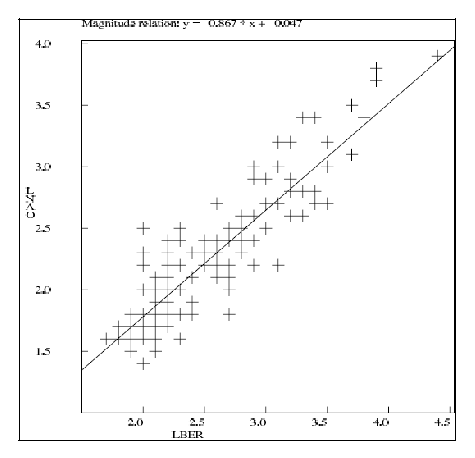
\includegraphics[width=0.9\linewidth]{fig/fig44}}
\caption{Example of using the MAG program. 
Relation between NORSAR and Bergen local magnitudes.}
%\label{fig:}
\end{figure}

An example of the \texttt{mag.par} parameter file: 

\verbatiminput{include/mag.par}

